\documentclass{article}
\usepackage{amsmath}
\usepackage{algorithm}
\usepackage[noend]{algpseudocode}
\usepackage{graphicx}
\usepackage{listings}
\usepackage[utf8]{inputenc}
\usepackage{array}
\usepackage{tabu}
\usepackage{color}
\usepackage{hyperref}
\usepackage{listings}
\usepackage{color}
 
\definecolor{codegreen}{rgb}{0,0.6,0}
\definecolor{codegray}{rgb}{0.5,0.5,0.5}
\definecolor{codepurple}{rgb}{0.58,0,0.82}
\definecolor{backcolour}{rgb}{0.95,0.95,0.92}
 
\lstdefinestyle{mystyle}{
    backgroundcolor=\color{backcolour},   
    commentstyle=\color{codegreen},
    keywordstyle=\color{magenta},
    numberstyle=\tiny\color{codegray},
    stringstyle=\color{codepurple},
    basicstyle=\footnotesize,
    breakatwhitespace=false,         
    breaklines=true,                 
    captionpos=b,                    
    keepspaces=true,                 
    numbers=left,                    
    numbersep=5pt,                  
    showspaces=false,                
    showstringspaces=false,
    showtabs=false,                  
    tabsize=2
}
 
\lstset{style=mystyle}


\hypersetup{
    colorlinks=true,
    linkcolor=blue,
    filecolor=magenta,      
    urlcolor=cyan,
    pdftitle={H20171030081 Report},
    bookmarks=true
}
 
\urlstyle{same}

\makeatletter
\def\BState{\State\hskip-\ALG@thistlm}
\makeatother
\graphicspath{ {./images/} }

\begin{document}


\paragraph{}
\begin{center}
\textbf{A Project Report }
\end{center}
\paragraph{}
\begin{center}
on 
\end{center}

\paragraph{}
\begin{center}
\textbf{\large{\textsl{Building Intrusion Detection System Based on the Analysis of Cowrie Honeypot Logs Using Elastic Search, Logstash ,Kibana ,Machine Learning Algorithms and VirusTotal }}}
\end{center}

\paragraph{}
\begin{center}
by 
\end{center}

\paragraph{}
\begin{center}
\textbf{SARADHI RAMAKRISHNA} \\
2017H1030081H \\
M.E Computer Science
\end{center}

\paragraph{}
\begin{center}
Under the supervision of \\
\textbf{CHITTARANJAN HOTA} \\
\textbf{RAJESH KUMAR SHRIVASTAVA }
\end{center}

\paragraph{}
\begin{center}
SUBMITTED IN FULFILMENT OF THE REQUIREMENTS OF \\
\textbf{BITS G540 RESEARCH PRACTICE}
\end{center}

\paragraph{}
\begin{center}

\includegraphics[scale=0.1]{bits_logo.png} 
\end{center}

\paragraph{}
\begin{center}
\textbf{BIRLA INSTITUTE OF TECHNOLOGY AND SCIENCE PILANI} \\
\textbf{HYDERABAD CAMPUS} \\
\textbf{(APRIL 2018) }
\end{center}

\thispagestyle{empty}
\newpage


\paragraph{}
\begin{center}
\textbf{\Large{ABSTRACT}}
\end{center}
\thispagestyle{empty}
\newpage 


\thispagestyle{empty}
 
\tableofcontents
 
\listoffigures
 
\listoftables

\lstlistoflistings

\newpage
 
\pagenumbering{arabic}

\section{Introduction of Tools}

\paragraph{}
In this section, i will be introducing the tools ,languages and API's which will be used throughout the report.

\subsection{ELK Stack}
\paragraph{}
"ELK" is the acronym for three open source projects: Elasticsearch, Logstash, and Kibana.

\subsubsection{Elastic Search}

\paragraph{}
Elasticsearch is a search engine based on Lucene. It provides a distributed, multitenant-capable full-text search engine with an HTTP web interface and schema-free JSON documents.

\subsubsection{Logstash}

\paragraph{}
Logstash is an open source tool for collecting, parsing, and storing logs for future use.

\subsubsection{Kibana}

\paragraph{}
Kibana is an open source data visualization plugin for Elasticsearch. It provides visualization capabilities on top of the content indexed on an Elasticsearch cluster. Users can create bar, line and scatter plots, or pie charts and maps on top of large volumes of data.

\subsection{Honeypots}

\paragraph{}
In computer terminology, a honeypot is a trap set to detect, deflect or in some manner counteract attempts at unauthorized use of information systems.

\paragraph{}
In other words, A server that is configured to detect an intruder by mirroring a real production system. It appears as an ordinary server doing work, but all the data and transactions are phony. Located either in or outside the firewall, these are used to learn about an intruder’s techniques as well as determine vulnerabilities in the real system.”

\paragraph{}
Based on design criteria, honeypots can be classified as

\begin{enumerate}
\item Low-interaction honeypots
\item Medium-interaction honeypots
\item High-interaction honeypots
\end{enumerate}

\subsubsection{Low-interaction honeypots}
\paragraph{}
Low-interaction honeypots simulate only the services frequently requested by attackers. Since they consume relatively few resources, multiple virtual machines can easily be hosted on one physical system, the virtual systems have a short response time, and less code is required, reducing the complexity of the security of the virtual systems.
\paragraph{}
Low-interaction honeypots present the hacker emulated services with a limited subset of the functionality they would expect from a server, with the intent of detecting sources of unauthorized activity. For example, the HTTP service on low-interaction honeypots would only support the commands needed to identify that a known exploit is being attempted.

\subsubsection{Medium-interaction honeypots}
\paragraph{}
Medium-interaction honeypots  might more fully implement the HTTP protocol to emulate a well-known vendor’s implementation, such as Apache. However, there are no implementations of a medium-interaction honeypots and for the purposes of this paper, the definition of low-interaction honeypots captures the functionality of medium-interaction honeypots in that they only provide partial implementation of services and do not allow typical, full interaction with the system as high-interaction honeypots.

\subsubsection{High-interaction honeypots}
\paragraph{}
High-interaction honeypots imitate the activities of the real systems that host a variety of services. It let the hacker interact with the system as they would any regular operating system, with the goal of capturing the maximum amount of information on the attacker’s techniques. Any command or application an end-user would expect to be installed is available and generally, there is little to no restriction placed on what the hacker can do once he/she comprises the system.
\paragraph{}
According to recent researches in high interaction honeypot technology, by employing virtual machines, multiple honeypots can be hosted on a single physical machine. Therefore, even if the honeypot is compromised, it can be restored more quickly. Although high interaction honeypots provide more security by being difficult to detect, but it has the main drawback that it is costly to maintain.

\subsubsection{Cowrie Honeypot}
\paragraph{}
Cowrie is used for our research purposes.Cowrie is a medium interaction SSH and Telnet honeypot designed to log brute force attacks and the shell interaction performed by the attacker.
\paragraph{Interesting Features of Cowrie Honeypot}

\begin{enumerate}
\item Fake filesystem with the ability to add/remove files. A full fake filesystem resembling a Debian 5.0 installation is included.
\item Possibility of adding fake file contents so the attacker can cat files such as /etc/passwd. Only minimal file contents are included.
\item Logging in JSON format for easy processing in log management solutions.
\end{enumerate}

\subsection{VirusTotal}
\paragraph{}
VirusTotal is a website created by the Spanish security company Hispasec Sistemas. Launched in June 2004, it was acquired by Google Inc. in September 2012. The company's ownership switched in January 2018 to Chronicle, a subsidiary of Alphabet Inc. (Google's parent company).

\paragraph{}
VirusTotal aggregates many antivirus products and online scan engines to check for viruses that the user's own antivirus may have missed, or to verify against any false positives.Files up to 256 MB can be uploaded to the website or sent via email.Anti-virus software vendors can receive copies of files that were flagged by other scans but passed by their own engine, to help improve their software and, by extension, VirusTotal's own capability. 

\subsubsection{List of Anti-Virus Engines used by VirusTotal}


\begin{table}[h!]
\begin{center}

\begin{tabular}{ |c|c|c|c| } 
 \hline
 AegisLab & Agnitum & AhnLab & Anity\\
 \hline
 Aladdin & Avast & AVG  & Avira \\
 \hline
 BluePex  & Baidu  & BitDefender & Bkav  \\
 \hline
 ByteHero & Quick Heal & CMC Antivirus & CYREN \\
 \hline
 ClamAV  & Comodo & CrowdStrike & Doctor Web Ltd. \\
 \hline
 Emsisoft & Endgame & Eset Software & Fortinet \\
 \hline
 F-Prot  & F-Secure & G Data & Hacksoft \\
 \hline
 Hauri  & IKARUS & nProtect & Invincea  \\
 \hline
 Jiangmin & K7AntiVirus & Kaspersky & Kingsoft\\
 \hline
 Malwarebytes  & McAfee & Microsoft & eScan \\
 \hline
 Nano Security  & Norman & Panda & Rising \\
 \hline
  Symantec  & VIPRE & TotalDefense & TrendMicro \\
 \hline
 
 
 \hline
\end{tabular}
\caption{List of Antivirus Engines}
\end{center}
\end{table}

\subsection{Github}
\paragraph{}
GitHub (originally known as Logical Awesome LLC) is a web-based hosting service for version control using git. It is mostly used for computer code. It offers all of the distributed version control and source code management (SCM) functionality of Git as well as adding its own features. It provides access control and several collaboration features such as bug tracking, feature requests, task management, and wikis for every project.

\paragraph{}
The code which is written for this project is entirely pushed to Github where it is bug free and version safe.

\section{Installation of Tools}
\paragraph{}
In this section, we will be mentioning about the installation of various tools which will be used in the project.

\subsection{Elastic Search}

\begin{enumerate}
\item Download the Debian Installation file from the below link \\
\textit{\href{https://www.elastic.co/downloads/elasticsearch}}
\item Install it using the below command \\
\textit{{\color{blue}iotsys3@iotsys3-Precision-Tower-3420:~} dpkg -i elastic-search-6.2.0.deb}
\item Now start the service using below command \\
\textit{{\color{blue}iotsys3@iotsys3-Precision-Tower-3420:~} sudo service elasticsearch start}
\end{enumerate}

\paragraph{}
Open the link \textit{http://localhost:9200} in the browser and check for the ouput which should look like below.

\begin{figure}[H]
\centering
\caption{Elastic Search Output}
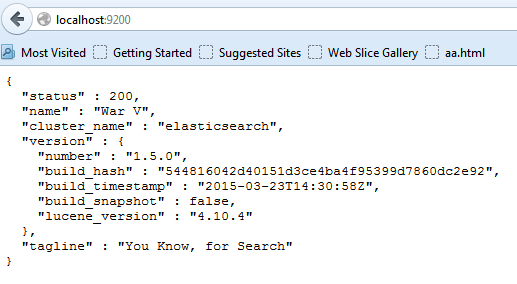
\includegraphics[scale=0.7]{Elastic_Search_Installation}
\end{figure}

\paragraph{}
We can check for the working of elastic search in the browser by typing the url \textit{http://localhost:9200} and verifying the output.

\subsection{Logstash}

\begin{enumerate}
\item Download the logstash debian installation file from below link\\
\textit{https://www.elastic.co/downloads/logstash}
\item Install it using the below command \\
\textit {{\color{blue}iotsys3@iotsys3-Precision-Tower-3420:~} dpkg -i logstash-6.2.2.deb}
\item Now start the service using below command\\
\textit{\color{blue}iotsys3@iotsys3-Precision-Tower-3420:~} sudo service logstash start
\end{enumerate}

\subsection{Kibana}

\begin{enumerate}
\item Download the Kibana debian installation file from below link\\
\textit{https://www.elastic.co/downloads/kibana}
\item Install it using the below command\\
\textit{{\color{blue}iotsys3@iotsys3-Precision-Tower-3420:~} dpkg -i kibana-6.2.2.deb}
\item Now start the service using below command\\
\textit{{\color{blue}iotsys3@iotsys3-Precision-Tower-3420:~} sudo service kibana start}
\end{enumerate}



\begin{figure}[H]
\centering
\caption{Kibana Dashboard}
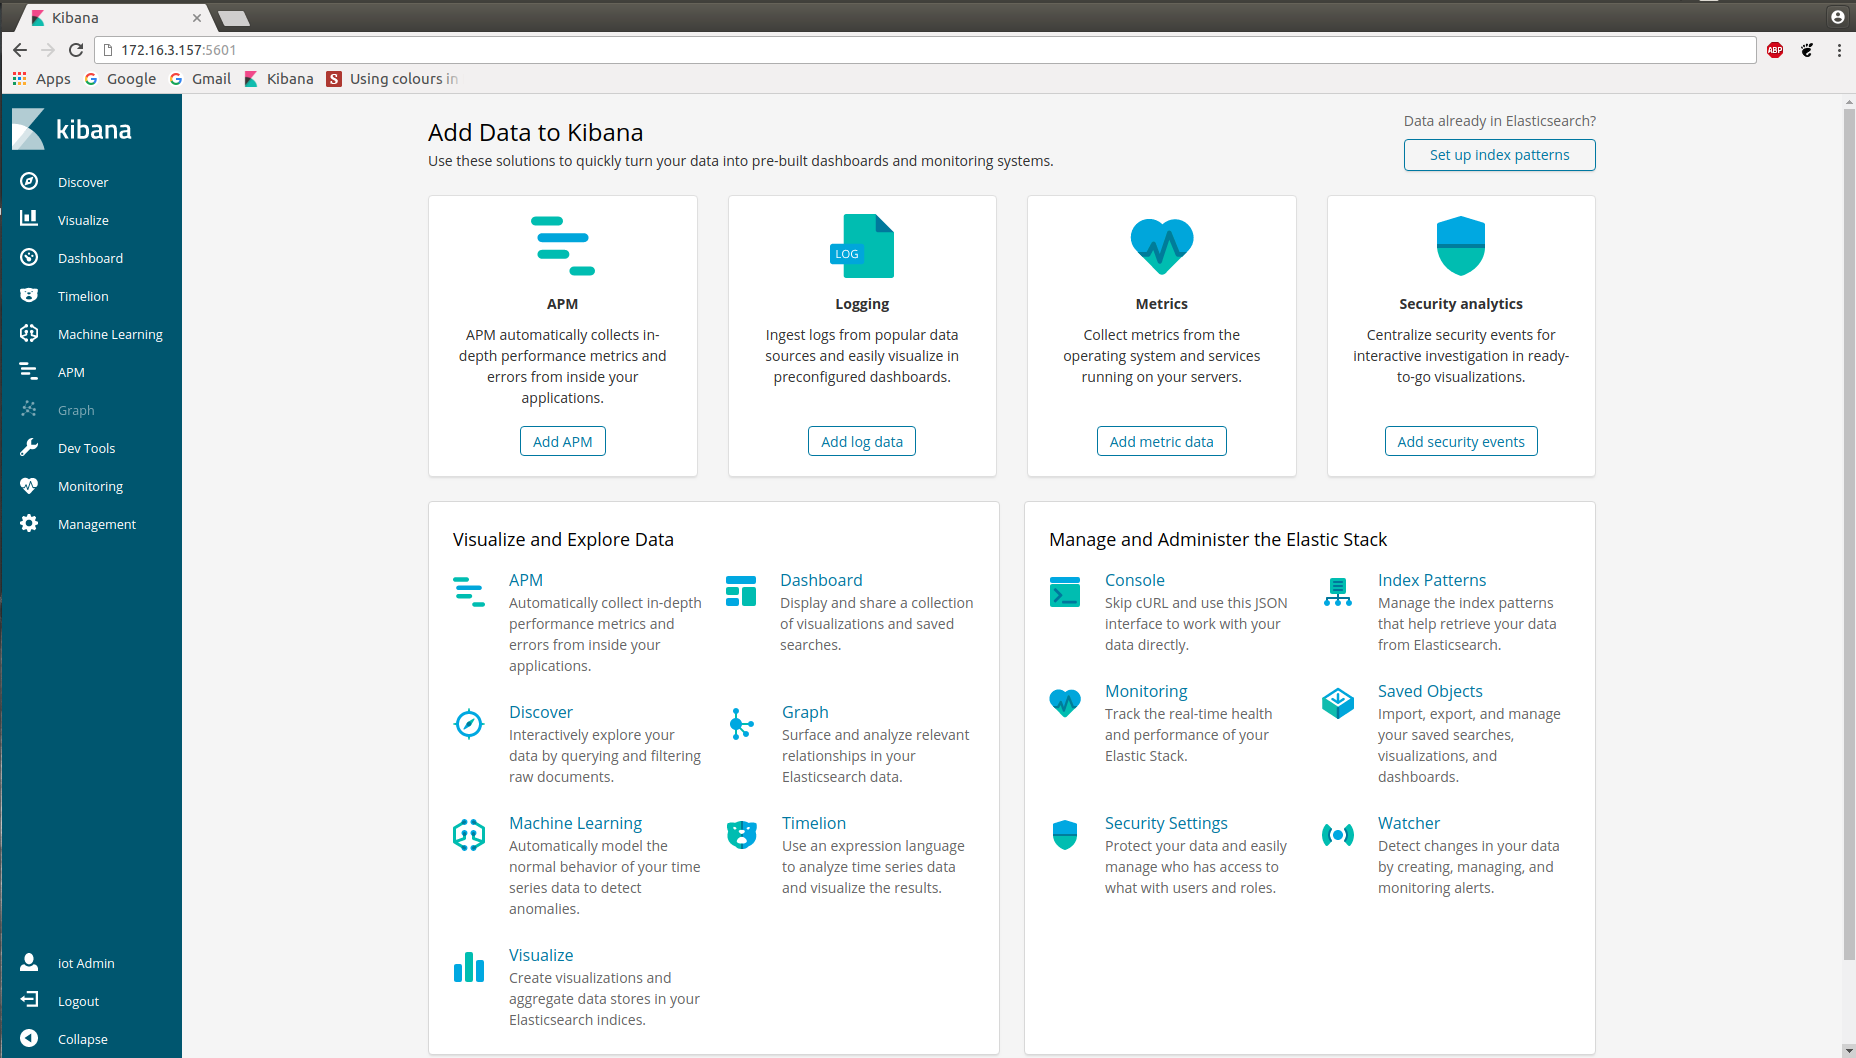
\includegraphics[scale=0.22]{Kibana_Installation}
\end{figure}

\paragraph{}
Open the link (\textit{http://localhost:5601}) in the browser and check for the Kibana Dashboard which looks like above.


\subsection{Cowrie Honeypot}

\paragraph{}
Cowrie honeypot is installed in a separate machine with public IP which is connected to the internet.It can be installed by following the steps given below.

\subsubsection{Install dependencies } 
\textit{{\color{blue}iotsys3@iotsys3-Precision-Tower-3420:} sudo apt-get install git python-virtualenv libssl-dev libffi-dev build-essential libpython-dev python2.7-minimal authbind}

\subsubsection{Create a user account } 
\textit{{\color{blue}iotsys3@iotsys3-Precision-Tower-3420:} sudo adduser --disabled-password cowrie}\\
\textit{{\color{blue}iotsys3@iotsys3-Precision-Tower-3420:} sudo su - cowrie}

\subsubsection{Checkout the code } 
\textit{{\color{blue}iotsys3@iotsys3-Precision-Tower-3420:} git clone http://github.com/micheloosterhof/cowrie}\\
\textit{{\color{blue}iotsys3@iotsys3-Precision-Tower-3420:} cd cowrie}


\subsubsection{Setup Virtual Environment } 
\textit{{\color{blue}iotsys3@iotsys3-Precision-Tower-3420:} pwd}\\
\textit{{\color{blue}iotsys3@iotsys3-Precision-Tower-3420:} virtualenv cowrie-env}

\subsubsection{Port redirection } 
\textit{{\color{blue}iotsys3@iotsys3-Precision-Tower-3420:} sudo iptables -t nat -A PREROUTING -p tcp --dport 22 -j REDIRECT --to-port 2222}

\paragraph{}
In the same folder, create a copy of \textit{cowrie.cfg.dist} and modify the file according to your needs like changing the name, SSH port number etc. 

\subsubsection{Starting Cowrie }
\textit{{\color{blue}iotsys3@iotsys3-Precision-Tower-3420:} bin/cowrie start}

\paragraph{}
Cowrie will be up and running on port 22 which will monitor all SSH logins and commands executed by the attackers or intruders.


\section{Working Model}

All the tools listed above are integrated to form a complete Working Model which looks like below.

\begin{figure}[H]
\centering
\caption{Working Model}
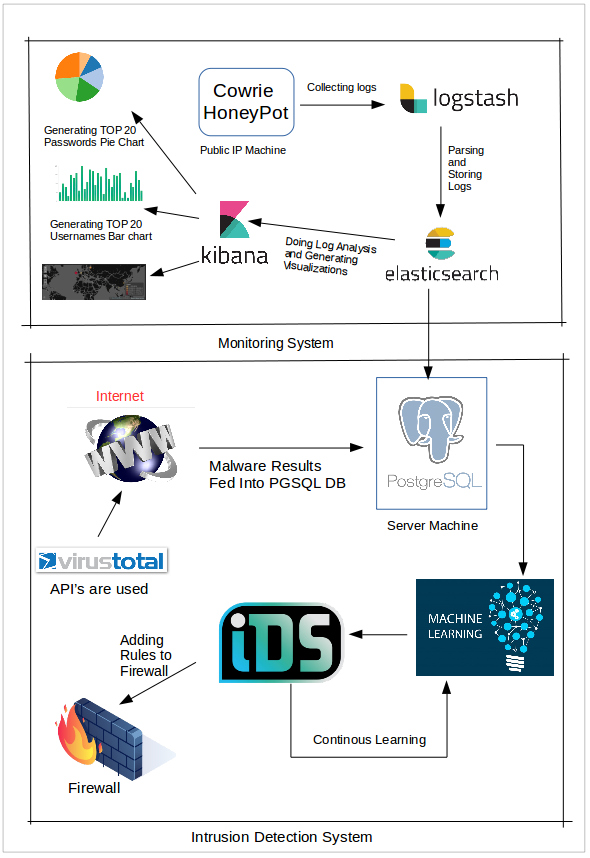
\includegraphics[scale=0.55]{Working_Model}
\end{figure}

\section{Monitoring System}

\begin{figure}[H]
\centering
\caption{Monitoring System}
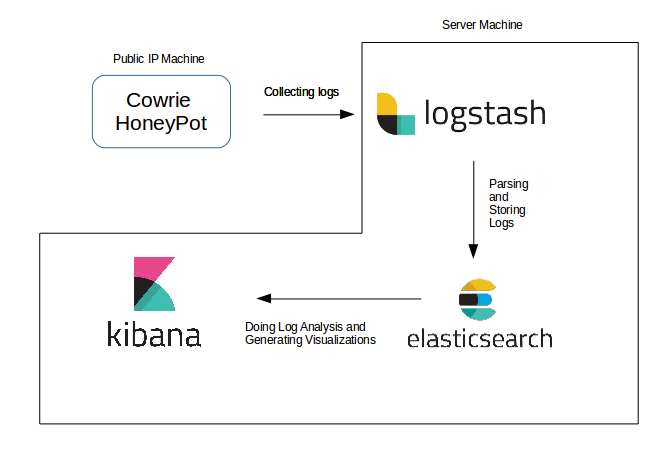
\includegraphics[scale=0.55]{Monitoring_System}
\end{figure}

\paragraph{}
Cowrie will be generating the logs in the form of JSON format which will be available in public IP machine as specified in the figure-3. In order to stream the logs from the public IP machine to Server machine, filebeat can be used which is an open source tool. Unfortunately we did not get to use that tool as there was no physical connection between public IP machine and server machine due to security reasons. 

\paragraph{}
So all the logs are copied from public IP machine to server machine on daily basis. These log files are supplied as input to Logstash which will parse, add metadata and push them to Elastic Search database. Logstash works on config files. Each config file has three parameters namely input, filter and output. Our config file is given below.

\lstinputlisting[language=python, caption=Cowrie Config File, captionpos=top]{cowrie.conf}

\begin{enumerate}
\item Input
\paragraph{}
It contains a parameter file which has options path, start-position and ignore-older. Path is where log files are present and start-position indicates from which point Logstash should start reading the logs from.
\item Filter
\paragraph{}
Filter is where entire processing happens in logstash. It has many options out of which json option is used as the logs are in JSON format. Some more information is added to the already present logs like country , Continent , latitude and longitude information which are specified in geoip option. Finally latitude and longitude are converted into float variables for plotting on map.
\item Output
\paragraph{}
It specifies options as to where the data should go after the processing is done. There are many options out of which we are using elastc search where data is stored in json format which will be in key value format.
\end{enumerate}

\paragraph{}
Data collected in the elastic search will be picked up by the Kibana by default as specified in the Kibana config files. Using the data visualizations are created for analyzing and monitoring the regular changes in data. Monitoring system was deployed for 40 days and collected nearly \textbf{2 Million Records}.

\paragraph{}
Using Kibana different visualizations are created which are listed below.
\begin{enumerate}
\item Daily Attacks Count Area Graph
\paragraph{}
An area graph was plotted against the count of attacks on daily basis. X-axis represents the date and Y-axis represents the count of attacks.It can observed that, attacks kept on increasing at the end.

\begin{figure}[H]
\centering
\caption{Daily Attacks Count Area Graph}
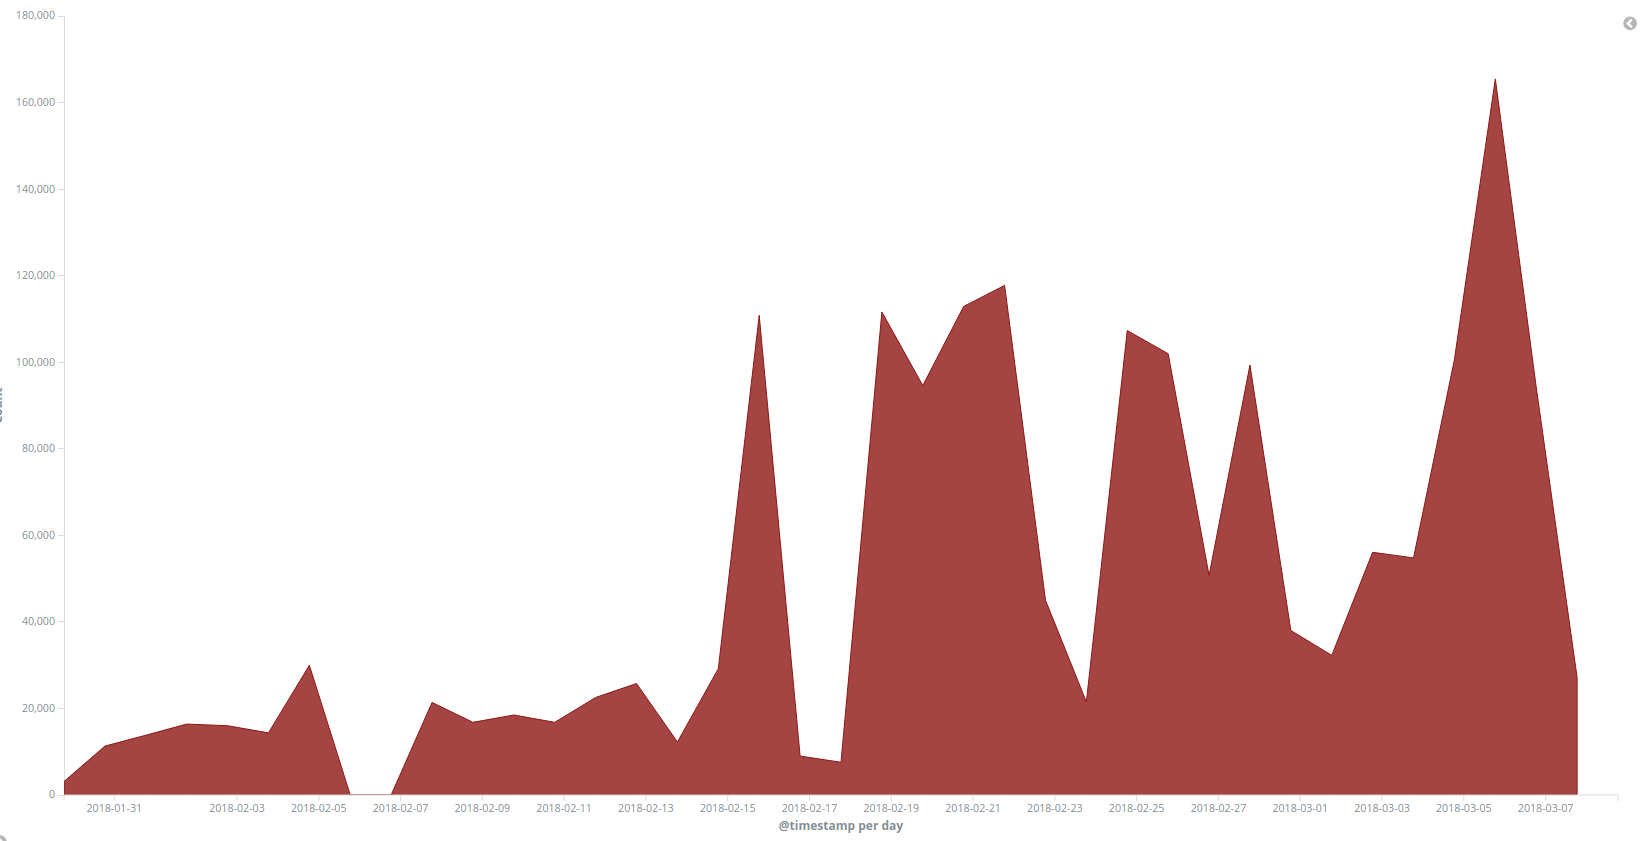
\includegraphics[scale=0.2]{Daily_Attacks_Count}
\end{figure}


\item Top 20 Usernames Histogram
\paragraph{}
A Histogram was used to represent the top 20 usernames that have been used by the attackers and intruders.

\begin{figure}[H]
\centering
\caption{Top 20 Usernames Histogram}
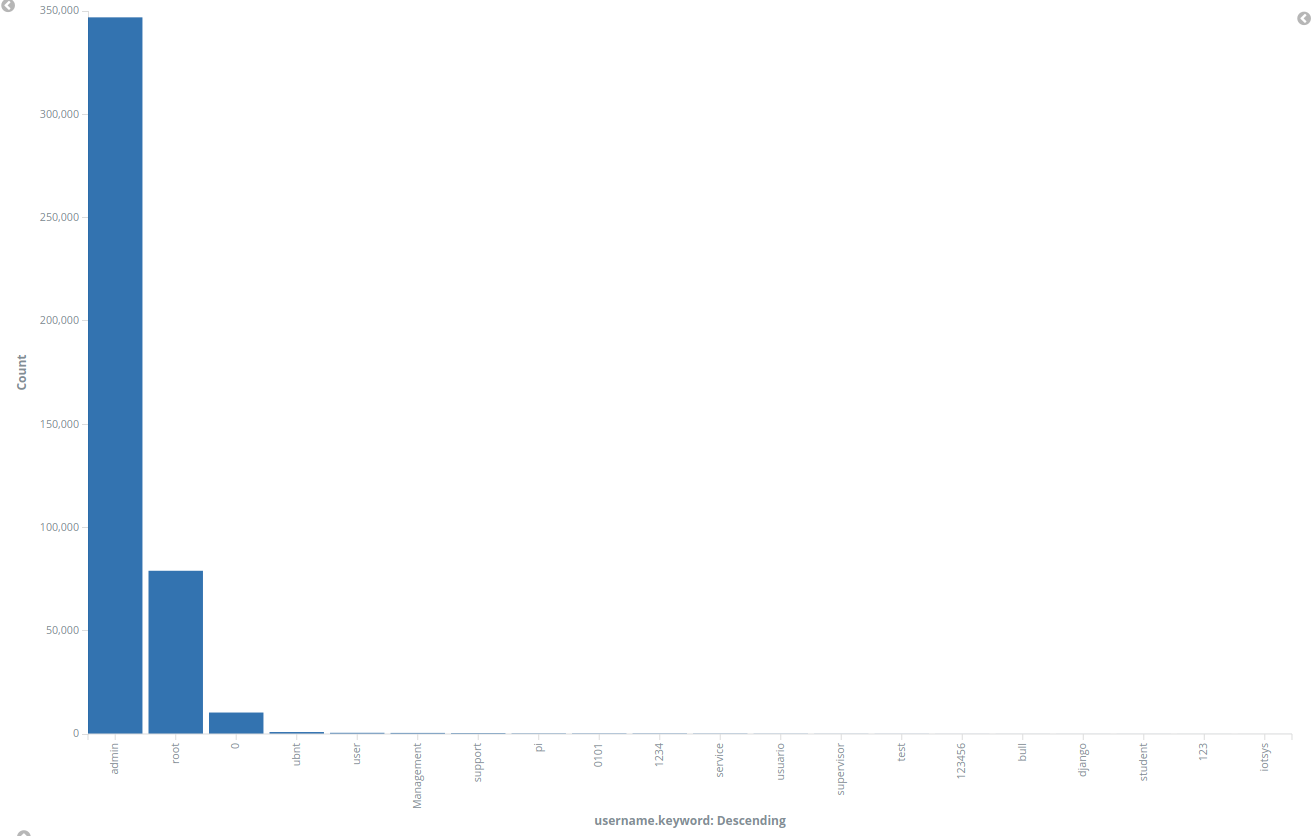
\includegraphics[scale=0.2]{Username_Histogram}
\end{figure}

\paragraph{}
From the graph, it can be observed that usernames "admin", "root and "ubnt" are mostly used by attackers.

\item Unique Count Of IP's
\paragraph{}
A Kibana Utility graph named Unique Count has been used for counting the Unique Number of IP's till now monitoring system has captured. It has found to be nearly 2000 IP's.

\begin{figure}[H]
\centering
\caption{Unique Count of IP's}
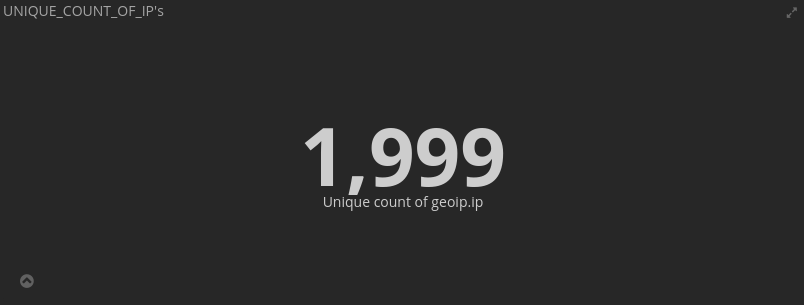
\includegraphics[scale=0.5]{Unique_IP}
\end{figure}

\item Top 20 Passwords Pie
\paragraph{}
A pie chart has been drawn against the top 20 passwords used by the attackers and intruders. It can be observed that passwords "ubnt" and "admin" are mostly used.

\begin{figure}[H]
\centering
\caption{Top 20 Passwords Pie}
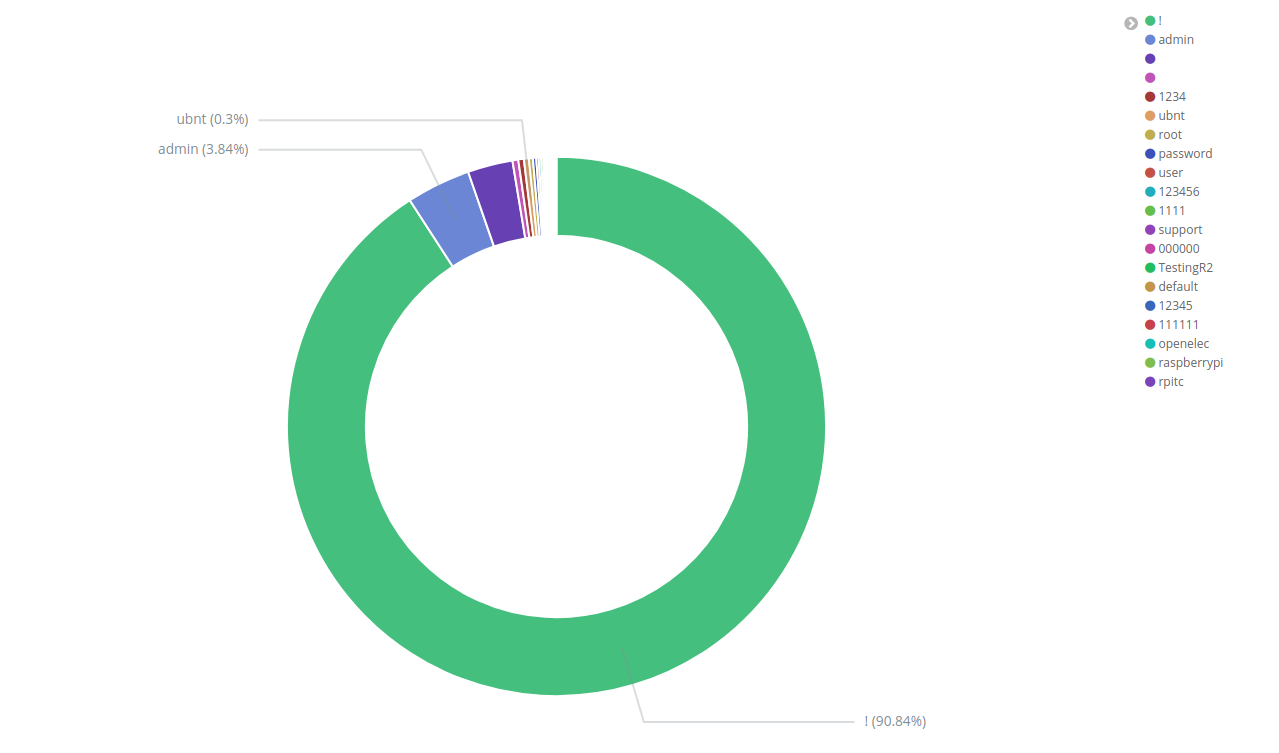
\includegraphics[scale=0.29]{Passwords_Pie}
\end{figure}

\item Global Attacks Map
\paragraph{}
A map is also plotted against the attacks receiving from different contries and continents using the latitude and longitude values. Most of the attacks are received from european continent and china country.

\begin{figure}[H]
\centering
\caption{Global Attacks Map}
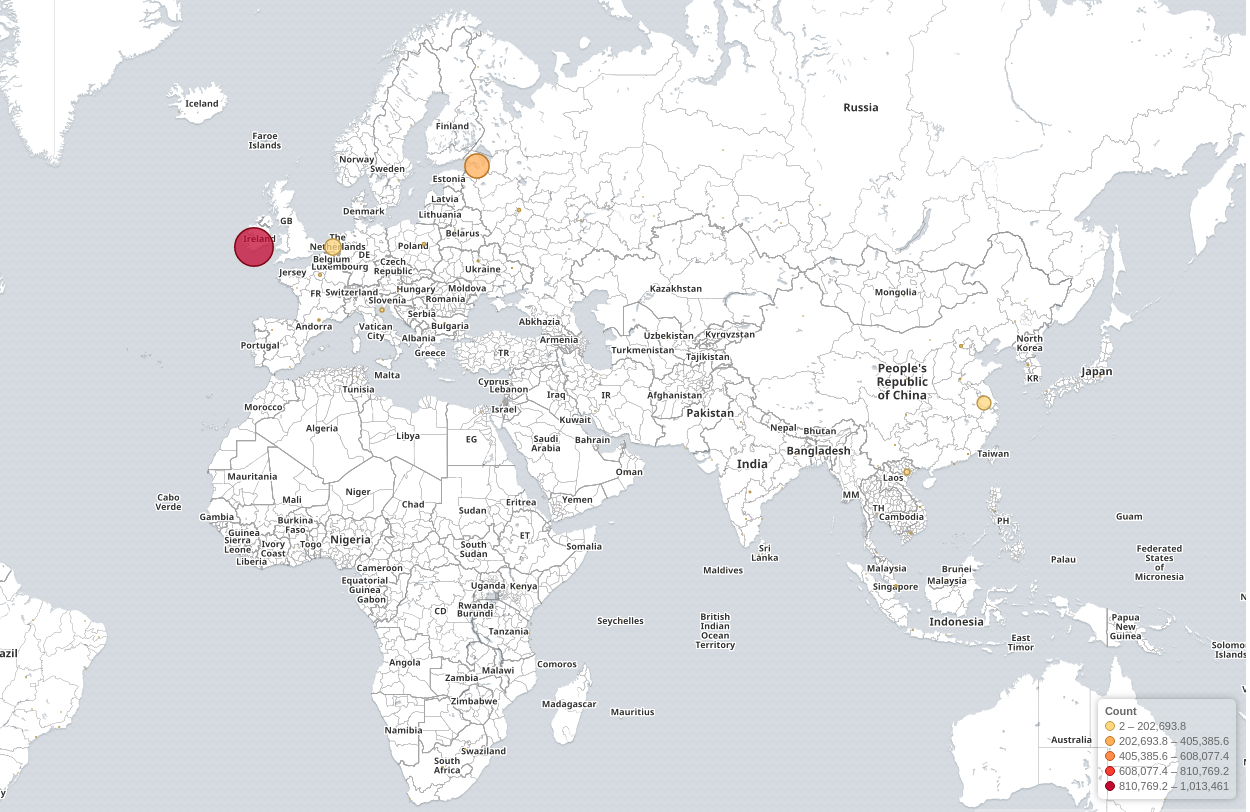
\includegraphics[scale=0.30]{Global_Attacks_Map}
\end{figure}

\end{enumerate}

\subsection{Stochastic Process}
\paragraph{}
Stochastic process is also called random process. It contains random variables with probabilities associated to it. While exact path cannot be inferred, assumptions can be made based on the probabilities of random variables. Attacks pattern observed is following random process or stochastic process as number of attacks on daily basis is not following any pattern.

\begin{figure}[H]
\centering
\caption{Stochastic Process}
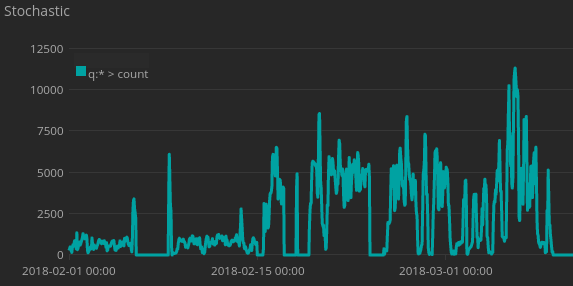
\includegraphics[scale=0.7]{Stochastic_Process}
\end{figure}

\section{Intrusion Detection System}
\paragraph{}
An Intrusion Detection System is a software application which regularly monitors the network for malicious activities and reports them to central authority for fail-safe measures. After the monitoring system is setup and data is collected , task is now to design an Intelligent Intrusion Detection System which applies machine learning algorithms on the data and comes up with firewall rules to block malicious activites and IP's. For designing, tools like VirusTotal API's, PostgreSQL database, Spark K-Means Algorithm etc. are used which is given below in detail.

\paragraph{}
Virus Total is a website where details about different malwares and IP's can be fetched by using their web interface or REST API's. For our convenience, API's are used to integrate with our python programs. Virus Total gives a normal user on an average of 1000 API requests per day combining malware samples and IP's. We have sent a mail to VirusTotal requesting Research User  privileges which has access to 10,000 API requests per day and all malware samples present in their database and got their approval.

\paragraph{}
In PostgreSQL, database named "cowrie" has been created and below tables were created to store the required data from Elastic Search and VirusTotal.

\begin{table}


\begin{tabular}{ |p{2cm}|p{5cm}|p{5cm}|  }
 \hline
 \textbf{S.No.} & \textbf{Table Name} & \textbf{Schema}\\
 \hline
 \hline
 1 & Dos-Attacks & public \\
 \hline
2 & Malicious-URLs & public \\
\hline
3 & Stats & public \\
\hline
\end{tabular}
 \caption{List of Tables in PostgreSQL Database}
\end{table}




\begin{figure}[H]
\centering
\caption{Intrusion Detection System}
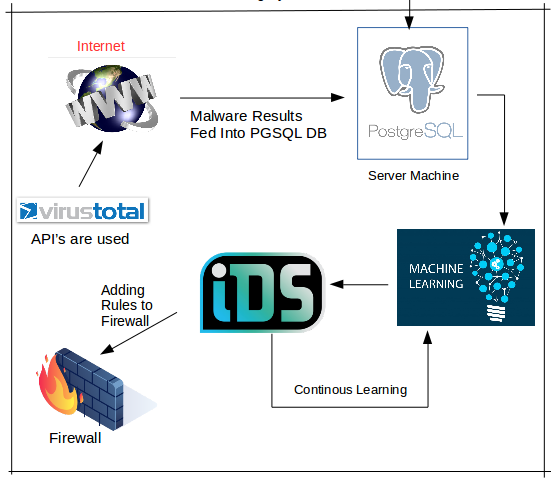
\includegraphics[scale=0.7]{Intrusion_Detection_System}
\end{figure}

\subsection{Malicious-URLs Table}

\begin{table}[H]
\begin{tabular}{ |p{2cm}|p{5cm}|p{5cm}|  }
 \hline
 \textbf{S.No.} & \textbf{Column Name} & \textbf{Column Datatype}\\
 \hline
 \hline
 1 & url & text \\
 \hline
2 & scan-url & text \\
\hline
3 & positives & integer \\
\hline
3 & total & integer \\
\hline
3 & identified-engines & text \\
\hline
\end{tabular}
 \caption{Schema of Malicious-URLs Table}
\end{table}

\paragraph{}
Column "url" is used to store the malicious url and "scan-url" is the ID to identify the job submitted to VirusTotal for malicious url. "positives" contains the number of antivirus engines identified the url as malicious and   "total" indicated the number of antivirus engines present in VirusTotal. "identified-engines" contains the names of all anti-virus engines. Malicious-urls table gets the data from VirusTotal API's. Python codes and their explanations are given below.

 
\lstinputlisting[language=python, caption=Get Malicious URLs From Virus Total, captionpos=top]{./files/12-GetMaliciousURLsFromIPsUsingVirusTotal.py}

 
\lstinputlisting[language=python, caption=Add URL's to PostgreSQL Database, captionpos=top]{./files/13-AddURLsToDB.py}

 
\lstinputlisting[language=python, caption=Submit URL's for Scan to VirusTotal, captionpos=top]{./files/14-SubmitURLsForScanUsingVirusTotal.py}

 
\lstinputlisting[language=python, caption=Get URL Scan results from VirusTotal, captionpos=top]{./files/15-GetURLScanResults.py}


\paragraph{}
Above python codes uses Virus Total API and sends requests for all the malicious urls identified for the specific IP. The response is decoded and then stored into the table. response looks like below.

\lstinputlisting[language=python, caption=Virus Total API Request Sample, captionpos=top]{./files/response.txt}

\paragraph{}
This response is parsed and requires fields are extracted to update the table in the database. These fields include "positives" which is the no of engines identified it as positive, "total" which is the count of the engines in total  and "identified-engines" which contains the names of all the engines in the response.


\subsection{Stats Table}

\begin{table}[H]
\begin{tabular}{ |p{2cm}|p{5cm}|p{5cm}|  }
 \hline
 \textbf{S.No.} & \textbf{Column Name} & \textbf{Column Datatype}\\
 \hline
 \hline
 1 & ip & character varying(20) \\
 \hline
2 & commands & text \\
\hline
3 & countofcommands & integer \\
\hline
4 & loginattempts & integer \\
\hline
5 & doscluster & text \\
\hline
6 & sentiment & integer \\
\hline
\end{tabular}
 \caption{Schema of Stats Table}
\end{table}

 
\paragraph{}
Column "IP" contains the ip of the attacker or intruder and "commands" contains all the commands executed by the attacker or the intruder till noe in cowrie honeypot. "Count-of-commands" contains the number of commands attacker executed. "login-attempts" contains the number of times attacker tried to login into the cowrie. "dos-cluster" contains the cluster number to which ip is clustered which will be updated dynamically. "sentiment" contains the value of ip which is updated after running machine learning algorithms.

\paragraph{}
All the python codes used for filling the table are given below one by one.


\lstinputlisting[language=python, caption=Get Unique IPs from Elastic Search, captionpos=top]{./files/01_GetUniqueIPs.py}

\paragraph{}
The above python code fetches all the IP's from elastic search, puts them in a set to avoid duplicates and copies all the IP's to the column named "ip" in Stats table. It uses the Elastic Search API's which looks like below.

\begin{lstlisting}[language=Python, caption=Elastic Search API Request Sample,captionpos=top]
POST localhost:9200/logstash-*/_search
{
  "size" : 0,
    "aggs" : {
        "distinct_ip" : {
            "cardinality" : {
              "field" : "geoip.ip"
            }
          
        }
    }
}
\end{lstlisting}


\lstinputlisting[language=python, caption=Get Commands Executed by IPs from Elastic Search, captionpos=top]{./files/02_GetCommandsForIPs.py}

\paragraph{}
The above python code fetches all the commands executed per IP , appends them together separated by semicolon and puts them in the column named "commands" in Stats table. It also updates the "countofcommands" column.

\lstinputlisting[language=python, caption=Get Login Attempts by IPs from Elastic Search, captionpos=top]{./files/03_getLoginAttemptsForIPs.py}

\paragraph{}
The above python code gets the number of login attempts done by each IP from the elastic search. It counts the attempts and stores them in column named "loginattempts" in Stats table. 

\subsubsection{DOS Attacks}
\paragraph{}
This "loginattempts" login is used to predict whether IP is performing DOS attack or not. For this , only those IP's are considered where after they log in , they don'e execute any commands and just leave. Spark K-Means Machine learning algorithm has been used to divide the IP's into 2 categories "High" and "Low". CSV file is generated  which is supplied as input to K-Means algorithm. Pseudo code is given below.

\lstinputlisting[language=python, caption=Generate Login Attempts in a CSV File, captionpos=top]{./files/04_GenerateLoginAttemptsCSV.py}

\lstinputlisting[language=python, caption=Applying Spark K-Means Algorithm, captionpos=top]{./files/05_K-Means.py}

\lstinputlisting[language=python, caption=Counting of DOS attacks, captionpos=top]{./files/06_countDOSAttacks.py}

\paragraph{}
After the above python file is executed, DOS attacks table looks like below.
Some IP's are also performing sniffing attacks where in they login and check for busybox utility.

\begin{table}[H]
\begin{tabular}{ |p{2cm}|p{5cm}|p{5cm}|  }
 \hline
 \textbf{S.No.} & \textbf{DOS Cluster} & \textbf{No. of IP's}\\
 \hline
 \hline
 1 & Severe & 16 \\
 \hline
2 & Medium & 5 \\
\hline
3 & Low & 1842 \\
\hline
\hline
 & \textbf{Total} & \textbf{1863} \\
\hline
\end{tabular}
 \caption{DOS Attacks Clustering Table}
\end{table}

\subsubsection{Modified Naive Bayes With K-Means for Classification}
\paragraph{}
Based on the commands executed by the IP, they have been classified into two classes as high and low using Modified Naive Bayes. As all the data is unlabeled , Sentiment analysis cannot be applied using original Naive Bayes.In modified naive Bayes, prior probability is assumed to be one as we have all data which belongs to only attack class. Effective algorithm is given below.

\lstinputlisting[language=python, caption=Modified Naive Bayes Algorithm Code, captionpos=top]{./files/07_Sentiment_Analysis.py}

\paragraph{}
After the application of Modified Naive Bayes, Posterior Probabilities are generated which are given as input to K-Means algorithm which groups them into clusters. Clusters are designed to be of two types naming high and low.
Based on the results, below table has been deduced.

\lstinputlisting[language=python, caption=K-Means Algorithm using Spark, captionpos=top]{./files/08_Sentiments_K_means.py}

\lstinputlisting[language=python, caption=K-Means Algorithm using Spark, captionpos=top]{./files/09_ClassifyIPs.py}





\begin{algorithm}[H]
\caption{Modified Naive Bayes With K-Means Clustering Algorithms}\label{euclid}
\begin{algorithmic}[1]

\State $\textbf{Probability}\textit{(IP is Malicious / Commands executed by IP }\text{) = }$
\begin{equation*}
  		\frac{\textbf{Probability}\textit{(IP is Malicious) * }\textbf{Probability}\textit{(Commands executed by IP / IP is Malicious)}}{\textbf{Probability}\textit{(Commands executed by IP)}}
	\end{equation*}
\State $\textbf{Note :}\textit{As we are working on Unclassified Data,We are assuming below values.}$
\State $\textbf{Probability}\textit{(IP is Malicious) = }\textbf{1} $
\State $\textbf{Probability}\textit{(Commands executed by IP) = }\textbf{1} $
\State $\textbf{Probability}\textit{(Commands executed by IP / IP is Malicious) = }$

\begin{equation*}
  		\frac{\textit{Frequency of Word + 1 (Smoothening Factor)}}{\textit{ Total Number of Words + Unique Number of Words}}
	\end{equation*}

\State $\textbf{Note :}\textit{ Commands executed by each IP is split into words and their }$
$\centerline{\textit{frequencies are stored in Database}}$
\State $\textit{Total No of Words} \gets \textit{N}$
\State $\textit{Unique No of Words} \gets \textit{dict}$
\While {$\textit{IP List} \textbf{ not } \textit{Empty} $}
	\State $\textit{No of Words} \gets \textit{Splitting Commands into words}$
	\State $\textbf{Probability}\textit{(IP is Malicious / Commands executed by IP }\text{)}$
	\State $\textbf{= Probability (}\textit{Commands executed by IP / IP is Malicious}) $ 
	\State $\textbf{= }\prod_{i=1}^{\textit{No of Words}}\textbf{Probability}\textit{(}\textit{Word}_i\textit{ in Command Executed/ IP is Malicious)}$
	\State $\textbf{= }\prod_{i=1}^{\textit{No of Words}}\frac{\textit{n}_i\textit{+ 1 }}{\textit{ N + dict}}$	
	
\EndWhile
\State $\textbf{done}$
\State $\textbf{Note : }\textit{ Each IP Final Probability will be stored in Database}$

\State $\textbf{Note : }\textit{After Storing the IP's Probabilities in Database,}\textbf{K-Means} $ $\textit{Clustering algorithm is applied to classify the IP's into two classes as high and Low.}$
 $\centerline{***********************************}$
 $\textbf{\centerline{K-Means is given below}}$
 $\centerline{***********************************}$
\State $\textbf{Input : }\textit{Set of Data Points }\textbf{D}\textit{ and No. of Clusters}\textbf{ K.}$
\State $\textbf{Output : }\textit{Cluster Centers that minimizes the squared error distortion.}$
\State $\textbf{Algorithm : }$
\begin{enumerate}
   \item \textit{Pick K Data points randomly from D to form cluster centers.}
   \item \textit{Assign each data point to its nearest cluster center by calculating and taking the minimum Euclidean Squared distance metric.}
   \item \textit{After all data points are assigned to their clusters,move each cluster center to mean of its assigned data points.}
   \item \textit{With new cluster centers, repeat 2 to 3 until there is no convergence.}
\end{enumerate}
\end{algorithmic}
\end{algorithm}


\begin{table}[H]
\begin{tabular}{ |p{2cm}|p{5cm}|p{5cm}|  }
 \hline
 \textbf{S.No.} & \textbf{Cluster Name} & \textbf{No. of IP's}\\
 \hline
 \hline
 1 & High & 136 \\
 \hline
2 & Low & 1842 \\
\hline
\hline
 & \textbf{Total} & \textbf{1978} \\
\hline
\end{tabular}
 \caption{Modified Naive Bayes and K-Means Results}
\end{table}

\subsubsection{DDOS Binaries}
\paragraph{}
Attackers who were able to login successfully has used their access to full effect by deploying the binaries and executable files on the machine and running them remotely whenever needed. Fortunately Cowrie happened to be a medium interaction honeypot which would not allow running any binaries or executable files. Some of the captured binaries are sent to VirusTotal and all of them are identified as serious DDos attacking binaries. Some of them are listed below.



\begin{table}[h!]
\begin{center}

\begin{tabular}{ |c|c|c|c| } 
 \hline
 ./lPg5Am8r & ./AObM55mP & ./ScDrDSSt & ./YL88yLHr\\
 \hline
 ./Tr5l603l & ./yu5LvV97 & ./VdPacLUl  & ./uzsiO4Hx \\
 \hline
 ./BRB3bpfb  & ./PWnQ7Tcn  & ./GgzxWgHv & ./zanTB34C  \\
 \hline
 ./udp4858 &  ./kEbIZq9x & ./MvlFggnh & ./6PcycAuj \\
 \hline
 ./o3e1ROxG  & ./b1fNqt0C & ./iUk3up10 & ./M7vu30G4 \\
 \hline
 ./KAFsqrpv & ./GYOIsFtx & ./tf2SD7fn &  \\
 \hline
\end{tabular}
\caption{List of DDos Binaries}
\end{center}
\end{table}

\paragraph{}
Some of the malicious URL's accessed by the attackers is captured by the cowrie. These are given below in the table.


\begin{table}[h!]
\begin{center}

\begin{tabular}{ |c| } 
 \hline
 http://www.bizqsoft.com/tp2/r6.log\\
 \hline
 http://185.165.29.196/lmao.sh\\
 \hline
 http://mdb7.cn:8081/exp  \\
 \hline
 http://203.146.208.208/drago/images/.ssh/y.txt \\
 \hline
 http://162.248.4.130/isu80 \\
 \hline
 https://doiaru.000webhostapp.com/zeni.txt  \\
 \hline
 http://61.147.112.10:1242/udp4858  \\
 \hline
 http://104.216.151.157/i3306m  \\
 \hline
  http://23.228.113.240/do3309  \\
 \hline
  http://23.228.113.240/ys808e  \\
 \hline
  http://14.142.118.25/m.sh  \\
 \hline
  http://107.189.130.20/ys808e  \\
 \hline
  http://192.200.218.166/g3308l  \\
 \hline
 
 
\end{tabular}
\caption{List of DDos Binaries}
\end{center}
\end{table}


\paragraph{}
Based on all the data listed above and tables created in PostgreSQL database and API's from VirusTotal, an intrusion detection system software has been developed which continously monitors the network where commands executed by any IP is noted and sent to the database built. If it is found in the database, it will be reported as malicious. If no information is found about the data in database, it keeps that in a separate column and keeps monitoring. If any anomaly is found, then the database will be updated with the new one. So it is a continous learning process for the software. Code is given below.

\lstinputlisting[language=python, caption=Intrusion Detection System Code, captionpos=top]{./files/16_IDS.py}

\begin{figure}[h!]
\centering
\caption{IP Identified as NOT Malicious by IDS}
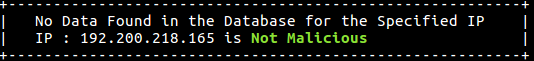
\includegraphics[scale=0.7]{IP_not_Malicious_IDS.png}
\end{figure}

\begin{figure}[h!]
\centering
\caption{IP Identified as Malicious by IDS}
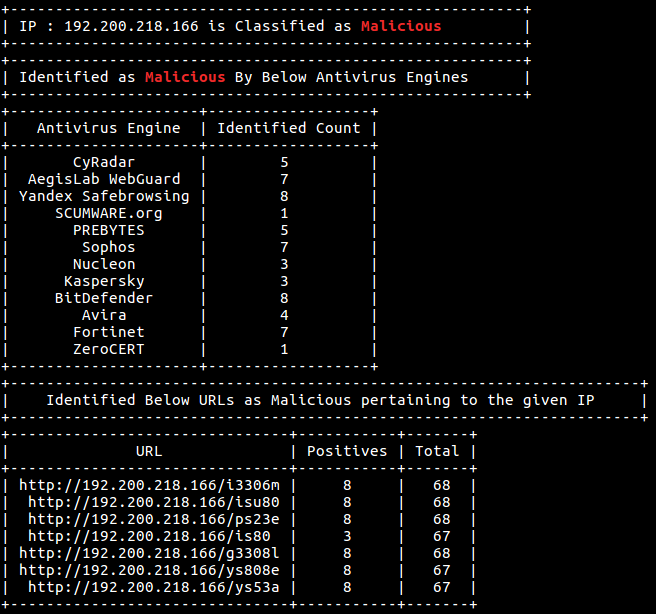
\includegraphics[scale=0.6]{IP_malicious_IDS.png}
\end{figure}

\paragraph{}
Based on the output from the IDS, firewall rules will be updated with the specific IP as blocking or nonblocking.

\paragraph{}
\textbf{Blocking : }\textit{iptables -A INPUT -s 192.200.218.166 -j DROP}

\paragraph{}
\textbf{Unblocking : }\textit{iptables -D INPUT -s 192.200.218.165 -j DROP}

\section{Conclusion}
In this report, we were able to figure out how vulnerable most of the internet devices are and what must be done in order to secure those devices. Recent developements in IOT has forced our hand to look at the security features at a microscopic level and improvements to be done. We have also tried to classify the different types of attacks on different IOT devices and on different ports. We have also tried to design a detection layer called Intrusion Detection System using all the historical and present data and were able to prevent if not detect some of those attacks.A lot has to be done in the security related work and hope everyone will put their hand towards acheiving it.


\begin{thebibliography}{9}



\bibitem{REF-1}
  Performance of ELK Stack and Commercial System in Security Log Analysis by \textit{ Sung Jun Son and Youngmi Kwon}
 
\bibitem{REF-2}
Building an IoT Data Hub with Elasticsearch, Logstash and Kibana by \textit{ Marcin Bajer}

\bibitem{REF-3}
Network security enhancement through effective log analysis using ELK by \textit{ Ibrahim Yahya Mohammed Al-Mahbashi and M. B. Potdar and Prashant Chauhan}

\bibitem{REF-4}

Malware capturing and detection in dionaea honeypot by \textit{ P Dilsheer Ali and T. Gireesh Kumar}

\bibitem{REF-5}

Integration of network intrusion detection systems and honeypot networks for cloud security by \textit{ Varan Mahajan and Sateesh K Peddoju}


\bibitem{REF-6}
  Honeynet Data Analysis and Distributed SSH Brute-Force Attacks by \textit{Gokul Kannan Sadasivam and Chittaranjan Hota and Anand Bhojan}
  
\bibitem{REF-7}
  Detection of Severe SSH Attacks using Honeypot Servers and Machine Learning Techniques by \textit{Gokul Kannan Sadasivam and Chittaranjan Hota and Anand Bhojan S}


\bibitem{REF-8}
  Classification of SSH attacks using Machine learning algorithms  by \textit{Gokul Kannan Sadasivam and Chittaranjan Hota and and Anand Bhojan}
  
\bibitem{REF-9}

IoT honeypot: A multi-component solution for handling manual and Mirai-based attacks by \textit{ Sasa Mrdovic and Haris Šemić}

\bibitem{REF-10}

Analysis of modern intrusion detection system by \textit{ Aleksey A. Titorenko and Alexey A. Frolov}

\bibitem{REF-11}
Clustering Approach Based on Mini Batch Kmeans for Intrusion Detection System Over Big Data by \textit{ Parisa Lotfallahtabrizi and Yasser Morgan}

\bibitem{REF-12}
Feature selection based intrusion detection system using the combination of DBSCAN, K-Mean++ and SMO algorithms by \textit{ Vandana Shakya and Rajni Ranjan Singh Makwana}


\bibitem{REF-13}

DDoS Attack Detection System: Utilizing Classification Algorithms with Apache Spark by \textit{ Amjad Alsirhani and Srinivas Sampalli and Peter Bodorik}

\bibitem{REF-14}

Testing of algorithms for anomaly detection in Big data using apache spark by \textit{ Sheeraz Niaz Lighari and Dil Muhammad Akbar Hussain}

\bibitem{REF-15}
Feature selection based intrusion detection system using the combination of DBSCAN, K-Mean++ and SMO algorithms by \textit{ Vandana Shakya and Rajni Ranjan Singh Makwana}


\bibitem{REF-16}

https://www.virustotal.com

\bibitem{REF-17}


Privacy and Security of Cloud-Based Internet of Things (IoT) by \textit{ Tanupriya Choudhury and Ayushi Gupta and Saurabh Pradhan and Praveen Kumar; Yogesh Singh Rathore}

\bibitem{REF-18}
Internet of Things (IoT) security platforms by \textit{ Ibrahim R. Waz and Mohamed Ali Sobh and Ayman M. Bahaa-Eldin}


\end{thebibliography}








\end{document}

